\begin{figure}[t]\label{fig:curve_1}
    \begin{subfigure}[b]{0.5\textwidth}\label{fig:curve_1_c_1}
        \centering
        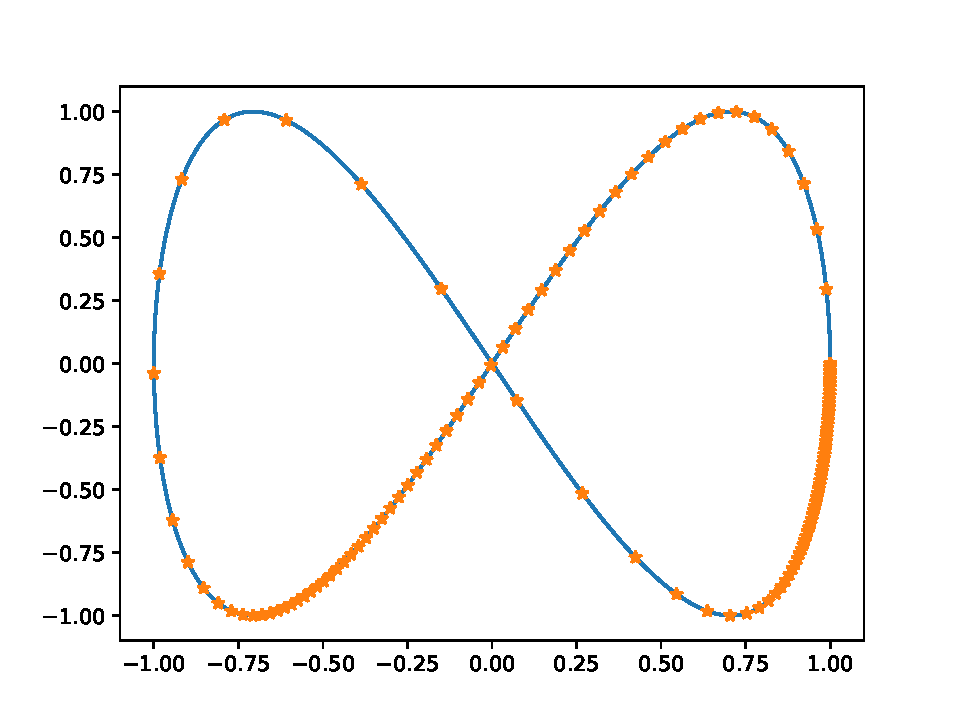
\includegraphics[width=\linewidth]{figures/curve_1/curve_c_1.pdf}
        \caption{\(c_1\)}
    \end{subfigure}
    \begin{subfigure}[b]{0.5\textwidth}\label{fig:curve_1_c_2}
        \centering
        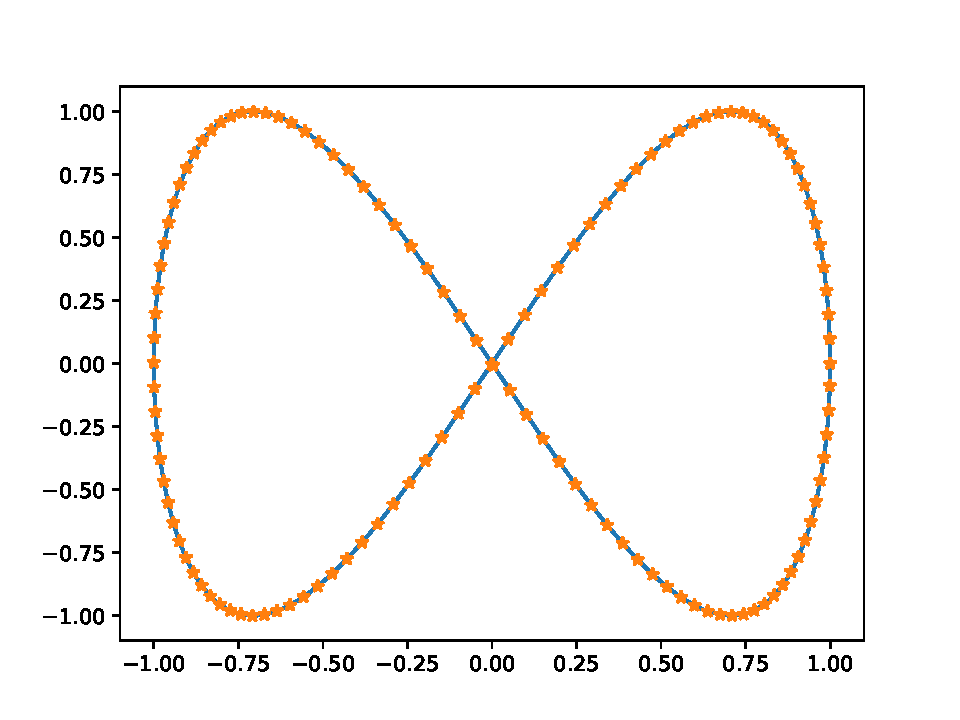
\includegraphics[width=\linewidth]{figures/curve_1/curve_c_2.pdf}
        \caption{\(c_2\)}
    \end{subfigure}
    \begin{subfigure}[t]{0.5\textwidth}\label{fig:curve_1_q}
        \centering
        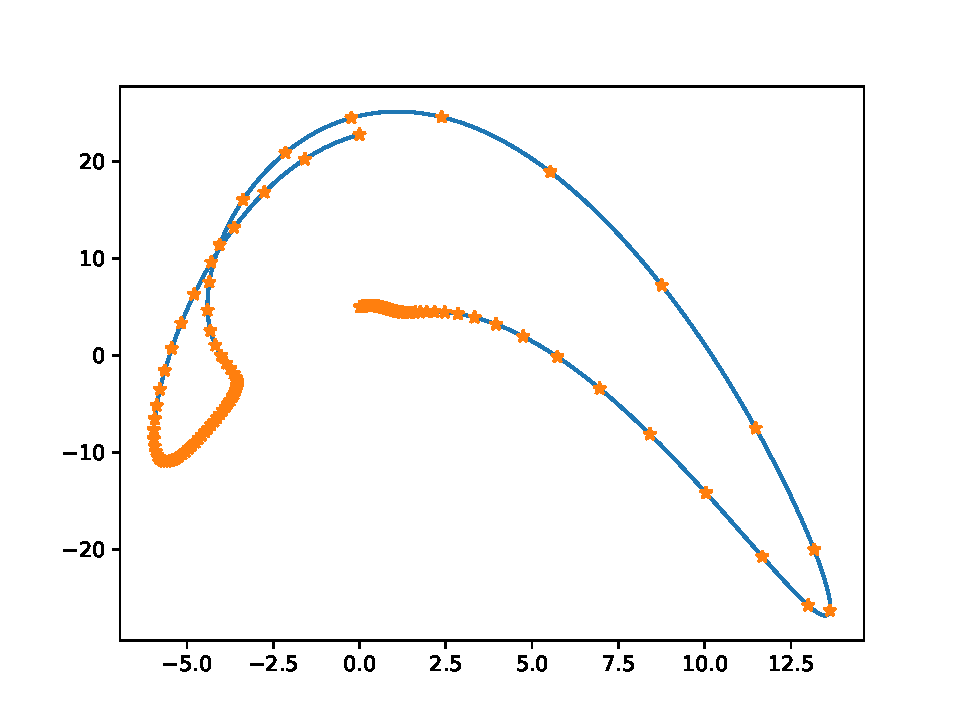
\includegraphics[width=\linewidth]{figures/curve_1/curve_q.pdf}
        \caption{\(q\)}
    \end{subfigure}
    \begin{subfigure}[t]{0.5\textwidth}\label{fig:curve_r}
        \centering
        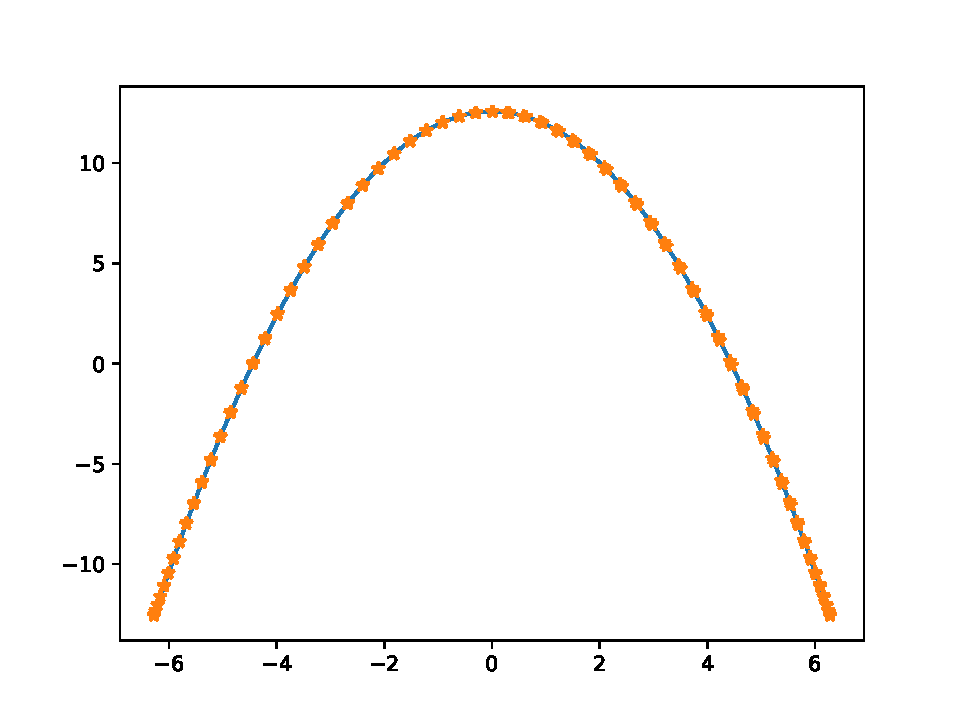
\includegraphics[width=\linewidth]{figures/curve_1/curve_r.pdf}
        \caption{\(r\)}
    \end{subfigure}
    \caption{The trajectory of \(c_1, c_2 \in \text{Imm}(I, \R^2)\), \(q = Q(c_1)\) and \(r = Q(c_2)\).}
\end{figure}

\begin{figure}[t]\label{fig:curve_1_example}
    \begin{subfigure}[t]{0.5\textwidth}\label{fig:curve_1_solution}
        \centering
        \includegraphics[width=\linewidth]{figures/curve_1/curve_1_exp_4/curve_1_exp_4_5_0.pdf}
        \caption{The approximate optimal reparametrization and the analytical solution.}
    \end{subfigure}
    \begin{subfigure}[t]{0.5\textwidth}\label{fig:curve_1_history}
        \centering
        \includegraphics[width=\linewidth]{figures/curve_1/curve_1_exp_4/history_curve_1_exp_4_5.pdf}
        \caption{The cost function \(L(\theta)\) with each iteration.}
    \end{subfigure}
    \caption{The approximate optimal reparametrization solution to test problem (1) with the corresponding loss history.}
\end{figure}

\begin{figure}\label{fig:curve_1_parmas_eks}
    \begin{subfigure}[t]{0.5\textwidth}
        \centering
        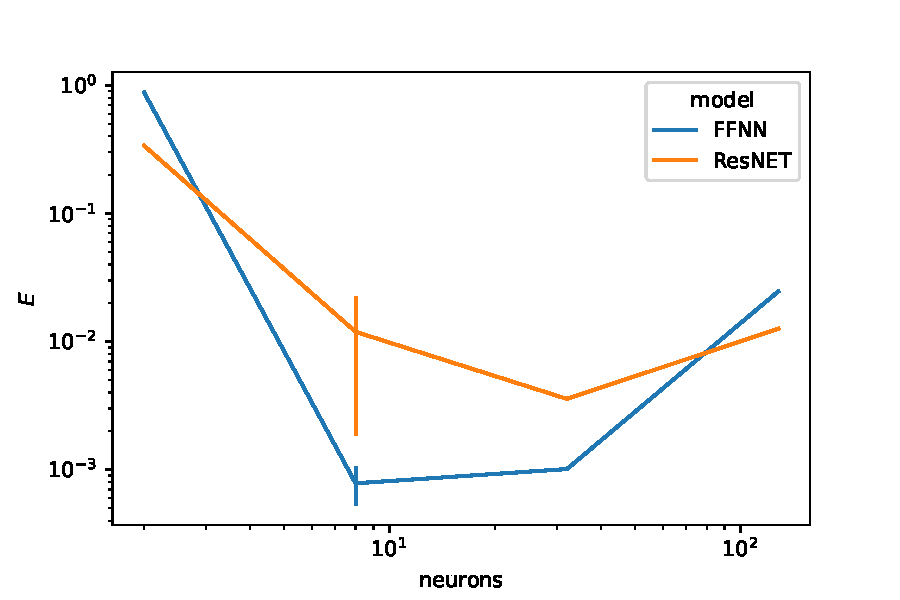
\includegraphics[width=\linewidth]{figures/curve_1/curve_1_exp_4/neurons_error.pdf}
        \caption{The final cost \(E\) with the number of neurons in each hidden layer.}
        \label{fig:curve_1_neuron_error}
    \end{subfigure}
    \begin{subfigure}[t]{0.5\textwidth}
        \centering
        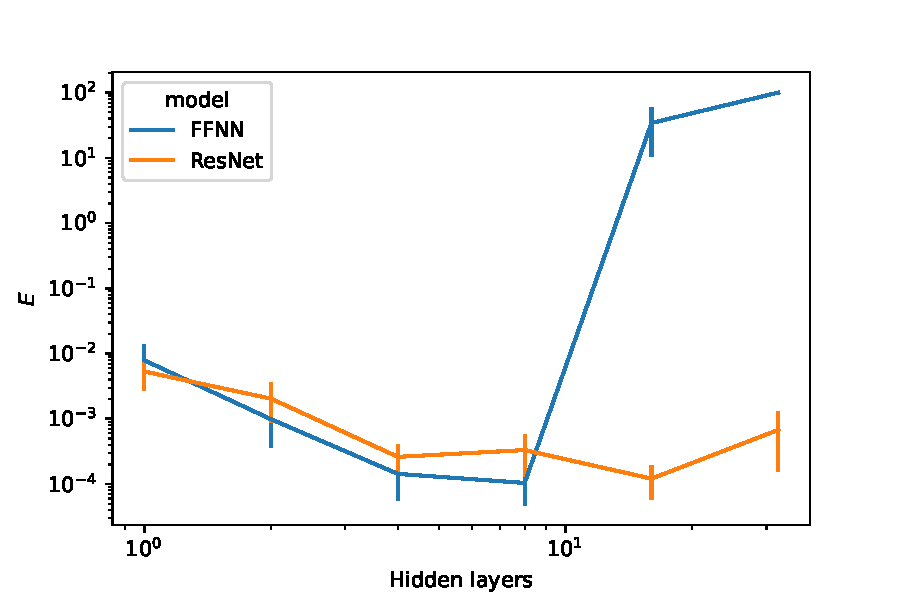
\includegraphics[width=\linewidth]{figures/curve_1/curve_1_exp_4/layer_error.pdf}
        \caption{Final cost \(E\) with the number of layers.}
        \label{fig:curve_1_layer_error}
    \end{subfigure}
    \caption{Result of ensemble training with different number of neurons and hidden layers. In Figure \ref{fig:curve_1_neuron_error} the number of layers was fixed at 2. In Figure \ref{fig:curve_1_layer_error} the number of neurons is fixed at 8 per hidden layer. The error bars denote a 80\% confidence interval found by bootstrapping.}
\end{figure}



\begin{tabular}{lrl}
    \toprule
    \(\bar{E} \) & Degrees of freedom & model         \\
    \midrule
    0.013143     & 34                 & ResNET        \\
    0.002253     & 9391               & ResNET        \\
    0.004567     & 30                 & Palais Layers \\
    0.000002     & 10000              & Palais Layers \\
    \bottomrule
\end{tabular}


Better structures and optimization algoritmhs for deeper networks.